%%%%%%%%%%%%%%%%%%%%%%%%%%%%%%%%%%%%%%%%%%%%%%%%%%%%%%%%%%%%%%%%%%%%%%%%%%%%%%%%
%%%%%%%%%%%%%%%%%%%%%%%%%%%%%%%%%%%%%%%%%%%%%%%%%%%%%%%%%%%%%%%%%%%%%%%%%%%%%%%%
%%                                                                            %%
%% This file contains the master thesis of Ossi Galkin. For more information  %%
%% look info page in the PDF.                                                 %%
%%                                                                            %%
%%%%%%%%%%%%%%%%%%%%%%%%%%%%%%%%%%%%%%%%%%%%%%%%%%%%%%%%%%%%%%%%%%%%%%%%%%%%%%%%
%%                                                                            %%
%% This is based latex template and uses aaltothesis.cls from Aaltothesis     %%
%% from Aaltothesis package. Available:                                       %%
%% https://wiki.aalto.fi/display/Aaltothesis/Aalto+Thesis+LaTeX+Template      %%
%%                                                                            %%
%% Aaltothesis is licensed under the terms of the MIT license below.          %%
%%                                                                            %%
%% See aaltothesis.cls for license text.                                      %%
%%                                                                            %%
%%%%%%%%%%%%%%%%%%%%%%%%%%%%%%%%%%%%%%%%%%%%%%%%%%%%%%%%%%%%%%%%%%%%%%%%%%%%%%%%
%%                                                                            %%
%% Official logos of Aalto University are used. Available:                    %%
%% https://wiki.aalto.fi/display/aaltolatex/Aalto+University+logo+package     %%
%% The aaltologo package has been published under Creative Commons            %%
%%  Attribution No-Derivative license                                         %%
%%                                                                            %%
%% See aaltologo.sty for license text.                                        %%
%%                                                                            %%
%%%%%%%%%%%%%%%%%%%%%%%%%%%%%%%%%%%%%%%%%%%%%%%%%%%%%%%%%%%%%%%%%%%%%%%%%%%%%%%%
%%%%%%%%%%%%%%%%%%%%%%%%%%%%%%%%%%%%%%%%%%%%%%%%%%%%%%%%%%%%%%%%%%%%%%%%%%%%%%%%
\documentclass[english, 12pt, a4paper, sci, utf8, a-2b, online, obeyspaces]{aaltothesis}
%\documentclass[english, 12pt, a4paper, elec, utf8, a-1b]{aaltothesis}
%\documentclass[english, 12pt, a4paper, elec, dvips, online]{aaltothesis}
%% Use the following options in the \documentclass macro above:
%% your school: arts, biz, chem, elec, eng, sci
%% the character encoding scheme used by your editor: utf8, latin1
%% thesis language: english, finish, swedish
%% make an archivable PDF/A-1b, PDF/A-2b or PDF/A-3b compliant file: a-1b,
%%                    a-2b, a-3b
%%                    (a normal pdf is produced without the a-*b option)
%% typeset in symmetric layout and blue hypertext for online publication: online
%%            (no option is the default, resulting in a wide margin on the
%%             binding side of the page and black hypertext)
%% two-sided printing: twoside (default is one-sided printing)
%%
%% Allow spaces inside command path obeyspaces is added. It goes to an url package.
\usepackage{graphicx}

%% Math fonts, symbols, and formatting; these are usually needed
\usepackage{amsfonts,amssymb,amsbsy}

%% https://www.johndcook.com/blog/2011/10/18/typesetting-c-in-latex/
\newcommand{\CS}{C\nolinebreak\hspace{-.05em}\raisebox{.6ex}{\scriptsize\bf \# }} 

\usepackage{listings}
\usepackage{csquotes}
\usepackage[all]{nowidow}

% add reference file
\usepackage[
backend=biber,
style=ieee, % originally was alphabetic
sorting=none % originally was ynt
]{biblatex}
\addbibresource{references.bib}

%% Change the school field to specify your school if the automatically set name
%% is wrong
% \university{aalto-yliopisto}
% \school{Sähkötekniikan korkeakoulu}
%% Edit to conform to your degree program
%%
\degreeprogram{Life Science Technologies}
%%
%% Your major subject
%%
\major{Complex Systems}
%%
%% Major subject code
%%
\code{SCI3060}
%%
%% Choose one of the three below
%%
%\univdegree{BSc}
\univdegree{MSc}
%\univdegree{Lic}
%%
%% Your name (self-explanatory...)
%%
\thesisauthor{Ossi Galkin}
%%
%% Your thesis title comes here and possibly again together with the Finnish or
%% Swedish abstract. Do not hyphenate the Title, and avoid writing too long a
%% title. Should LaTeX typeset a long title unsatisfactorily, you might have to
%% force a line break using the \\ control characters.
%% In this case...
%% Remember, the Title should not be hyphenated!
%% A possible "and" in the Title should not be the last word in the line, it
%% begins in the next line.
%% Specify the Title again without the linebreak characters in the optional
%% argument in box brackets. This is done because the Title is part of the 
%% metadata in the pdf/a file, and the metadata cannot contain line breaks.
%%
\thesistitle{Enterprise Application Integration Architecture Recovery}
%\thesistitle[Title of the thesis]{Title of\\ the thesis}
%%
%%
\place{Espoo}
%%
%% The date for the bachelor's thesis is the day it is presented
%%
\date{21.5.2019}
%%
%% Thesis supervisor
%% Note the "\" character in the Title after the period and before the space
%% and the following character string.
%% This is because the period is not the end of a sentence after which a
%% slightly longer space follows, but what is desired is a regular interword
%% space.
%%
\supervisor{Prof.\ Mikko Kivelä}
%%
%% Advisor(s)---two at the most---of the thesis. Check with your supervisor how
%% many official advisors you can have.
%%
%\advisor{Prof.\ Pirjo Professor}
\advisor{M.Sc. (Tech.) Minttu Mustonen}
%\advisor{MSc Sarah Scientist}
%%
%% Aaltologo: syntax:
%% \uselogo{aaltoRed|aaltoBlue|aaltoYellow|aaltoGray|aaltoGrayScale}{?|!|''}
%% The logo language is set to be the same as the thesis language.
%%
\uselogo{aaltoBlue}{!}
%%
%% The English abstract:
%% All the details (name, Title, etc.) on the abstract page appear as specified
%% above.
%% Thesis keywords:
%% Note! The keywords are separated using the \spc macro
%%
\keywords{System Integration, Software Architecture Recovery, Orchestration Architecture Recovery}
%%
%% The abstract text. This text is included in the metadata of the pdf file as well
%% as the abstract page.
%%
%\thesisabstract{
%Hand written abstract to metadata.
%}
%% Copyright text. Copyright of work is with the creator/author of the work
%% regardless of whether the copyright mark is explicitly in work or not.
%% You may, if you wish, publish your work under a Creative Commons license (see
%% creaticecommons.org), in which case the license text must be visible in the
%% work. Write here the copyright text you want. It is written into the metadata
%% of the pdf file as well.
%% Syntax:
%% \copyrigthtext{metadata text}{text visible on the page}
%% 
%% In the macro below, the text is written in the metadata must have a \noexpand
%% macro before the \copyright special character, and macros (\copyright and
%% \year here) must be separated by the \ character (space character) from the
%% text that follows. The macros in the argument of the \copyrighttext macro
%% automatically insert the year and the author's name. (Note! \ThesisAuthor is
%% an internal macro of the aaltothesis.cls class file).
%% Of course, the same text could have simply been written as
%% \copyrighttext{Copyright \noexpand\copyright\ 2018 Eddie Engineer}
%% {Copyright \copyright{} 2018 Eddie Engineer}
%%
\copyrighttext{Copyright \noexpand\copyright\ \number\year\ \ThesisAuthor}
{Copyright \copyright{} \number\year{} \ThesisAuthor}
%% You can prevent LaTeX from writing into the xmpdata file (it contains all the 
%% metadata to be written into the pdf file) by setting the writexmpdata switch
%% to 'false'. This allows you to write the metadata in the correct format
%% directly into the file thesistemplate.xmpdata.
%\setboolean{writexmpdatafile}{false}
%% All that is printed on paper starts here
%%

\pdfinfo{
   /Author (\ThesisAuthor)}

\begin{document}
%% Create the cover page
%%
\makecoverpage
%% Typeset the copyright text.
%% If you wish, you may leave out the copyright text from the human-readable
%% page of the pdf file. This may seem like an attractive idea for the printed
%% document especially if "Copyright (c) yyyy Eddie Engineer" is the only text
%% on the page. However, the recommendation is to print this copyright text.
%%
\makecopyrightpage
%% Note that when writing your thesis in English, place the English abstract
%% first followed by the possible Finnish or Swedish abstract.
% Aalto logo should be random so change it :D
\uselogo{aaltoRed}{?}
%% Abstract text
%% All the details (name, Title, etc.) on the abstract page appear as specified
%% above.
%%

\begin{abstractpage}[english]
Large and medium-sized enterprise has multiple business applications, such as customer relations management (CRM) and enterprise resource planning (ERP) software. Business applications need data from each other, but they rarely communicate with each other out of the box. An enterprise application integration (EAI) platform is used to tie them together. Automating communication between business applications is called orchestration. As EAI is used to implement communication between business applications, in theory, it could be used to map the architecture of the orchestration layer. As companies evolve, so does the software they use. Either documentation is never done, or it is not updated. Overall, the frequent problem is that the company loses track of what software systems it has and how they are used. 

This work studies the feasibility of building software that can automatically recover orchestration architecture. The orchestration architecture is then represented as a network to enable further analysis and visualization. This research investigates whether it is possible to use that network to detect business applications that are being used and whether the production environment is separate from the testing environment. In addition, those nodes connecting the testing, and production environments are determined.

The results suggest that it is possible to detect orchestration architecture automatically. Because of a unique characteristic of orchestration layer implementation, such a model can outperform more general architecture recovery models. With a recovered architecture, it is possible to detect whether the production environment is separate from the testing environment and to identify connecting nodes. However, used applications were not discovered using modularity optimization.


\end{abstractpage}
%% The text in the \thesisabstract macro is stored in the macro \abstractext, so
%% you can use the text metadata abstract directly as follows:
%%
%\begin{abstractpage}[english]
%    \abstracttext{}
%\end{abstractpage}
%% Force a new page so that the possible Finnish or Swedish abstract does not
%% begin on the same page
%%
\newpage
% Aalto logo should be random so change it :D
\uselogo{aaltoYellow}{''}
%%
%% Abstract in Finnish.  Delete if you don't need it. 
%%
\thesistitle{Järjestelmäintegraation arkkitehtuurin palauttaminen}
\advisor{DI Minttu Mustonen}
\degreeprogram{Life Science Technologies}
%\department{Elektroniikan ja nanotekniikan laitos}
\major{Complex Systems}
%% The keywords need not be separated by \spc now.
\keywords{Järjestelmäintegraatio, Ohjelmistoarkkitehtuurin palautus, orkestraatioarkkitehtuurin palautus}
%% Abstract text
\begin{abstractpage}[finnish]
Suurilla ja keskisuurilla organisaatioilla on useita liiketoimintaohjelmistoja, kuten asiakkuudenhallinta- ja toiminnanohjausohjelmistoja. Yritysohjelmistot tarvitsevat tietoja toisiltaan, mutta ne harvoin kommunikoivat keskenään käyttövalmiina. Järjestelmäintegraatioalustaa käytetään ohjelmistojen yhdistämiseksi. Liiketoimintaohjelmistojen välisen viestinnän automatisointia kutsutaan orkestroinniksi. Koska järjestelmäintegraatiota käytetään viestinnän toteuttamiseen liiketoimintaohjelmistojen välillä, sitä voidaan käyttää orkestrointikerroksen arkkitehtuurin kartoittamiseen. Yritysten kehittyessä myös niiden käyttämät ohjelmat kehittyvät. Usein niitä ei joko dokumentoida ollenkaan tai dokumentaatio jää päivittämättä. Kaiken kaikkiaan yleinen ongelma on se, että yritys menettää tiedon siitä, mitä ohjelmistoja sillä on ja miten niitä käytetään.

Tässä työssä tarkastellaan ohjelmiston toteuttamista, joka voi automaattisesti palauttaa orkestraatioarkkitehtuurin. Arkkitehtuuri esitetään verkostona, joka mahdollistaa lisäanalyysin ja visualisoinnin. Lisäksi selvitetään: Onko mahdollista käyttää tätä verkostoa yrityksen käyttämien liiketoimintasovellusten tunnistamiseksi. Onko tuotantoympäristö erillään testausympäristöstä. Näiden lisäksi määritetään mitkä järjestelmät yhdistävät kehitys-, testaus- ja tuotantoympäristöjä.

Tuloksista voidaan päätellä, että on mahdollista palauttaa orkestrointiarkkitehtuuri ohjelmallisesti. Orkestrointikerroksen toteutuksen ominaisuuksien vuoksi toteutettu malli suoriutui paremmin kuin yleiset arkkitehtuurin palautusmallit. Palautetun arkkitehtuurin avulla on mahdollista havaita, onko tuotantoympäristö erillinen testausympäristöstä ja tunnistaa liitäntäsolmut. Käytettyjä sovelluksia ei kuitenkaan löydetty modulaarisuuden optimoinnin avulla, joka oli työssä käytetty klusterointi menetelmä.


\end{abstractpage}
%% Preface
%%
\mysection{Preface}
%\mysection{Esipuhe}

The work for this thesis was carried out in HiQ Finland Ltd. I would like to thank the company for the opportunity to write this thesis. 

I would like to thank my supervisor Professor Mikko Kivelä, and my instructor M.Sc. (Tech.) Minttu Mustonen for their guidance during the working on this thesis. In addition, I would also thank all of those who have contributed to work. Especially, I want to thank M.Sc. (Tech.) Erkka Honkavaara, B.Sc. (Econ. \& Bus. Adm.) Atso Galkin, B.Eng. Pekka Kinnunen and M.Sc. (Tech.) Sakari Castrén for their support at multiple points during the process writing this thesis and implementing the model.

I want to express my gratitude to my friends and family and everyone I forget to mention by name for their support and encouragement. Finally, I would like to thank the love of my life, Essi Pitkänen, for being compassionate, patient and supporting for all this time.

\vspace{5cm}
Otaniemi, \today

\vspace{5mm}
{\hfill Ossi Galkin \hspace{1cm}}
%% Force a new page after the preface
%%
\newpage
%% Table of contents. 
%%
\thesistableofcontents
%% Symbols and abbreviations
\mysection{Abbreviations and Acronyms} 
\begin{tabular}{ll}
ASCII   & American Standard Code for Information Interchange \\
API     & Application Programming Interface \\
AMQP    & Advanced Message Queuing Protocol \\
BI      & Business Intelligence \\ 
BPMN    & Business Process Model and Notation \\ 
COBOL   & Common Business-Oriented Language \\
CSV     & Comma-Separated Values \\
DLL     & Dynamically Linking Library \\
EAI     & Enterprise Application Integration \\
EDI     & Electronic Data Interchange \\
ERP     & Enterprise Resources Planning \\
ESB     & Enterprise Service Bus \\
FTP     & File Transfer Protocol \\
FTPS    & FTP Over Secure Sockets Layer (SSL) \\ 
GUID    & Globally Unique IDentifier \\
HTTP    & Hyper Text Transfer Protocol \\
HTTPS   & Hyper Text Transfer Protocol Secure \\
IT      & Information Technology \\
JSON    & JavaScript Object Notation \\
POSIX   & Portable Operating System Interface \\
SaaS    & Software as a Service \\
SOA     & Service oriented architecture \\
SOAP    & Simple Object Access Protocol \\
Regex   & A Regular Expression, sometimes shortened to Regexp \\
REST    & Representational State Transfer \\
SFTP    & Secure Shell (SSH) File Transfer Protocol \\
SNMP    & Simple Network Management Protocol \\
SQL     & Structured Query Language \\
UI      & User Interface \\
UNC     & Uniform Naming Convention \\
URI     & Uniform Resource Identifier \\
URL     & Uniform Resource Locator \\
VAN     & A value-added network \\
WWW     & World Wide Web \\
XML     & Extensible Markup Language
\end{tabular}

%% \clearpage is similar to \newpage, but it also flushes the floats (figures
%% and tables).
%%
\cleardoublepage
%% Text body begins. Note that since the text body is mostly in Finnish the
%% majority of comments are also in Finnish after this point. There is no point
%% in explaining Finnish-language specific thesis conventions in English.
%% This text will be translated into English soon.
%%

\section{Introduction}
\label{sec:introduction}
%% Leave page number of the first page empty
%% 
\thispagestyle{empty}
Most large and medium-sized enterprises tend to have dozens of different computer systems. Connecting these systems so they can share data and business processes is called enterprise application integration (EAI) or integration for short. The integration enables enterprises to use their systems together to enable business processes. For integration, enterprises typically utilize a special software system called an integration platform. Integration platforms are designed to be efficient to attach other systems through a wide range of communication protocols. They have the means to modify the format of data, for example. Other systems usually provide only a limited means for integration (e.g., they might have only a limited application programming interface (API) or no interfaces at all). Moreover, these systems are not usually directly compatible with other systems. Usually, the format of the data varies in different systems. In addition, EAI platforms provide visibility and monitoring capabilities to integrations. As companies acquire more systems, the number of data flows, and automations between them grow. Automation of business processes, computer systems, and software is called orchestration, which also forms the integration layer that delivers data between computer systems.

As companies grow and evolve, the software they utilize has been changing. Unnecessary legacy systems are deactivated or migrated to new systems. New systems and individual interfaces are introduced. The computer system keeps evolving with the company. With this, the widespread problem is that a company loses track of what software systems are utilized and how they are used. That is due to the failure to thoroughly document new systems or because the company forgets to add to a list of software being acquired. Documentation also needs updating. Otherwise, the documentation becomes outdated or contains systems that are no longer present. Therefore, companies lose information regarding how and what computer systems are being used. 

Software architecture recovery is a process where the architecture-level information is formed from a system implementation. Architecture recovery has not been previously applied to integration architecture. However, a specific characteristic of an integration orchestration layer should help to recover its architecture compared to software in general.

\subsection{Problem Statement and Scope}
The aim of this thesis is to develop software that can recover the integration architecture from an implemented integration orchestration. In addition, this is fulfilled without using any documentation about the implemented orchestration. Software architecture recovery is generally known to pose a problem without a proper solution. However, this thesis studies whether the unique properties of an integration platform can be utilized to recover the integration architecture. Miniservice, as an architecture of the integration layer, makes it possible to recover architecture. Connections to other systems are easily detected from the parameters of the integration flow.

Hierarchical clustering is applied to a network to group different integration endpoints to the same system. The resulting architecture is represented as a network. The properties of the network are compared to the known properties of a scale-free network. Furthermore, different methods of integration, such as spaghetti integration are explored.

The main aim of this work is to recover the orchestration architecture. Once the architecture is known, it is briefly analyzed to detect the business applications adopted by the company. Additionally, the network is analyzed to detect whether the production environment is separate from the testing environment. If it is not separate, then production might depend on systems intended only for testing and therefore might lack monitoring or other elements required from the production environment. In addition, nodes connecting the environments are identified. Furthermore, it is investigated whether it is possible to use that network to detect business applications that are being used.

In this work, only architecture is recovered. Any analysis of the traffic in the integration is not performed. However, it would be possible to combine information regarding the integration architecture to traffic logs. It should also be highlighted that the goal is not to recover the architecture of the used EAI platform. The goal is to recover the architecture of the integration layer built on top of EAI platform (i.e., the architecture of the orchestration layers). Furthermore, the architecture is not recovered for processes connected to the message buses or message queue.

The method is tested using integrations built for a Finnish company that operates in the energy industry. As they have automated large parts of their business, their integration architecture contains highly sensitive business information; therefore, only a brief description of the analysis of the resulting network is provided. In addition, they wished not to be named. The integration is built on top of the FRENDS hybrid integration platform~\cite{hiq2018frends}.

\subsection{Thesis Structure}

Chapter~\ref{sec:background} presents a literature review on integrations and software architecture recovery. In addition, several principles that have been proposed and tried regarding how to combine several software systems are examined. Furthermore, the impact of the hybrid cloud to integrations is briefly considered. Chapter~\ref{sec:product_frends} will give an overview of product FRENDS and how they affect integration architecture recovery. Chapter~\ref{sec:methods_of_integration} discuss expected properties of recovered architecture and how standard network analyzing techniques can be exploited to investigate resulting network. 

Chapter~\ref{sec:methodology} gives an overview of the methodology used in this work, that is platform independent. The methodology consists of filtering the data, Clustering connections with hierarchical clustering, and searching the connections from implemented integrations with pattern matching. Chapter~\ref{sec:powerbi_model_and_r} expands previous Chapter with details of implemented Power Bi model.

Chapter~\ref{sec:analysis} contains the results and analysis for the network that represents the orchestration architecture from the customer's data that was used to test recovery methods. Chapter~\ref{sec:summary} presents the conclusions of the results of this thesis.

%% In a thesis, every section starts a new page, hence \clearpage
\clearpage

\section{Background}
\label{sec:background}

\subsection{Enterprise Application Integration}
\label{sec:enterprise_application_integration}
Information systems are usually built so that they focus on only the data and business processing in their domains. They can also provide only a limited interface due to a lack of standards~\cite{song2008research}. Thus, information sharing between these information systems becomes unavailable. The integration works by connecting these, enabling information sharing between them and enabling them to co-operate.

With well-integrated systems, enterprises can quickly respond to the changing environment. That provides the possibility to utilize all existing systems with greater agility. When the data from all systems are available, they enable faster development of new business processes with reduced costs~\cite{finkelstein2006enterprise}.

A single software can have coherent design principles, applying only selected concepts~\cite{brooks1995the}. When two or more systems are integrated, this is not generally possible, as existing systems can have different design concepts~\cite{garlan1995architectural}~\cite{garlan2009architectural}. Therefore, when the data from multiple systems are utilized, the data typically needs to be transformed thoroughly to be utilized appropriately.

As companies grow, evolve, and develop, the software they operate evolve with them. Old unnecessary systems are deactivated or migrated to new systems, and individual interfaces are deprecated. New systems are developed, while the old systems are removed. Overall, computer systems keep evolving with the company~\cite{garlan1995architectural}~\cite{garlan2009architectural}.

Integration works by moving data from where they are to where they are needed in the right form. Thus, building a common data model or transformation between the existing models is a significant challenge for any software~\cite{aiken1996data}~\cite{estublier2000software} and especially integration software. As Land~\cite[p. 338]{land3003software} stated: \textquote{The evolution, migration, and integration of existing software (legacy) systems are widespread and a formidable challenge to today's businesses.} 

Like all other software fields, EAI platforms are continually evolving. Despite this, some concepts and technologies have ever-increasing importance and form the basis for which most integration platforms have been built. According to Hohpe~\cite{hohpe2004enterprise}, they address three fundamental challenges that all integration solutions must deal with: slow, and unreliable networks, the fact that any two applications are different, and that change is inevitable.

\subsection{Terminology}
The terminology for discussing integration \textit{strategies}, \textit{patterns}, \textit{techniques}, \textit{technologies}, \textit{topology}, \textit{architecture}, and \textit{methods} is not entirely established. The terms are often used interchangeably, as they are closely related. In this thesis, they are used in the same way as Hohpe has defined them~\cite{hohpe2004enterprise}. Integration \textit{strategies} and \textit{technologies} are the technological basis on which integration is built. Integration strategies are discussed in Section~\ref{sec:integration_strategies}.  Integration \textit{architecture}, \textit{patterns}, \textit{methods}, \textit{techniques}, and \textit{topology} indicate how systems are integrated and connected. Integration methods are discussed in Chapter~\ref{sec:methods_of_integration}.

\subsection{Integration Strategies}
\label{sec:integration_strategies}
In all the following strategies, it is common that data are stored in a different format in different systems~\cite{hohpe2004enterprise}. Therefore, integration must transform or map data from the format of the writer to that of the reader. In practice, mapping is usually the most time-consuming and thus expensive part of a file transfer. 

\subsubsection{File transfer}
Applications can share data via files. The data is written in the file and then delivered where it is needed. The applications must agree on file location, name, and format as well as which will delete the file if necessary and the timing when the file is created. Mainframe computers usually use file systems based on common business-oriented language (COBOL) conventions, whereas Unix and Windows-based systems use flat files, comma-separated values (CSV), JavaScript Object Notation (JSON) or Extensible Markup Language (XML) files. Multiple file transfer techniques have been developed, such as electronic data interchange (EDI) files over a virtual area network (VAN) and File Transfer Protocol (FTP), FTP Over SSL (FTPS) and SSH File Transfer Protocol (SFTP) over the internet. File transfer is often used because it makes integration simple, as integration has only to transfer files. However, it requires that both the writer of the file and its reader agree on the file format. When this is not achieved, transformation must be done in the integration. 

\subsubsection{Shared databases}
When many applications share the same database, no data needs be transferred from one application to another because there are no duplicate data. The significant difficulty of the shared database is that it is incredibly difficult and often impossible for many software vendors to agree on the data schema and format of the data. When applications are distributed across many locations, access to the database across a network is typically too slow to be practical. Distributing databases allows applications to connect via the local network but raises an issue regarding the computer on which the data should be saved. In addition, resolving locking conflicts on the distributed database can quickly become a performance disaster.

\subsubsection{Remote procedure invocation }
Remote procedure invocation, also known as remote procedure call (RPC), allows one system to expose functionality so that it can be accessed remotely from other systems. If the system must modify data from other systems or perform something, it does so by calling other applications. This allows each application to maintain the integrity and its data format. Furthermore, the application can change its data format without alternating other applications. Multiple technologies, such as Simple Network Management Protocol (SNMP), SSH, .NET Remoting, and Java EMI, implement remote procedure invocation. Nowadays, methods are usually based on nearly universal internet standards, such as Simple Object Access Protocol (SOAP), on which Web Services-Management is based, for example. 

\subsubsection{Messaging}
Messages from an application are published to a common message channel. Applications must agree on the channel and format so that messages can be read from the channel later. Compared to file transfers, messaging is more immediate. Compared to shared databases, it is better encapsulated. Moreover, compared to the remote process invocation, it is more reliable. However, it requires a more complex programming model and adds overhead to the communication. In addition, it might have synchronization issues or be unavailable due to limited platform support and could result in vendor lock-in after implementation. Messaging systems can be further divided into different parts: send and forget messaging and store and forward messaging~\cite{zimmermann2016decade}. Most new methods count as messaging, such as service buses, queues, and multiple internet-based techniques, such as SOAP, Representational State Transfer (REST), Message Queuing Telemetry Transport, and Advanced Message Queuing Protocol (AMQP). 

\subsection{Cloud and Hybrid Cloud Computing}
The traditional method for enterprise to acquire information technology (IT) assets, hardware, and software is to buy them and maintain them internally. In other words, they use on-premises software. Cloud computing is changing this. Resources, IT assets, hardware, and software are being rented as a service from service providers. Usually, companies move gradually toward the cloud. They have some systems installed on-premises and other in the cloud (i.e., they have a hybrid cloud). Hybrid clouds bring a unique set of advantages and disadvantages, as discussed in this chapter.

A hybrid cloud is a cloud-computing environment that combines on-premises, private cloud, or public cloud services~\cite{microsoft2018cloud}~\cite{microsoft2018what}. To enable data sharing between them, orchestration is a necessity. The hybrid cloud gives roughly the same benefits as the single public cloud, such as the ability to grow computing resources as demand grows, but it also prevents giving third parties complete access to the databases and their data. Enterprises gain the flexibility of the public cloud while keeping critical business and sensitive data on premises. The hybrid cloud also provides scalability by eliminating the need to make capital investments when acquiring computing resources. It also makes it possible to free those resources when they are no longer used, which provides cost efficiency. In addition, it is possible to move less sensitive computing to the cloud, freeing up local resources for more sensitive data and applications. According to Won~\cite{kim2009adoption,} large and medium-sized enterprises face eight types of issues prevent moving to cloud computing: outage (availability), security, performance, compliance, private clouds, integration, cost, and the environment.

In addition to traditional integration challenges, discussed in Section~\ref{sec:enterprise_application_integration}, cloud integration provides a few unique advantages and challenges. The challenges include security, data integrity, API limitations, data mapping complexity, and talent shortage~\cite{mulesoft2018understanding}~\cite{hildebrand2018top}. Like other cloud applications, cloud integration provides scalability in terms of end users and the number of applications. It also enables faster integration to software as a service (SaaS) applications and enables faster development and deployment~\cite{mungrah2017cloud}.

Cloud integration is built on existing standards and protocols, such as SOAP and HTTP (i.e., REST~\cite{jin2009research}). Therefore, it is easy to add new connections to applications. Cloud integration provides a more straightforward and more flexible integration that is easier to design, develop, and maintain compared to a traditional EAI.

\subsection{Software Architecture Erosion}
\label{software_architecture_erosion}
Software architecture erosion is a term describing the difference between planned or desired architecture and the actual architecture of the implemented software~\cite{terra2012recommending}. Software architecture erosion occurs during natural software evolution, when plans are not followed, or when implementation details violate the principles of the selected architecture~\cite{perry1992foundations}. This can be a result of a lack of knowledge of the desired architecture or more often a result of too few resources to fully implement a solution that fulfills the architecture preferences rather than just something that works. Modifications are not necessarily documented entirely, and the resulting documentation can become inconsistent or incomplete as the code changes. Software architecture erosion is sometimes also referred to as technical debt. However, that term also refers to old solutions whose architecture is coherent, but that is old and no longer preferred.

\subsection{Software Architecture Archaeology in General}
\label{sec:software_architecture_archaeology_in_general} 
Software architecture recovery is a process to extract a high-level architectural model from the available system implementation~\cite{rasool2007software}. Terms such as \textit{reverse architecting} ~\cite{krikhaar1997reverse} or \textit{architecture reconstruction} ~\cite{ducasse2009software} are also used. Legacy systems become obsolete with time because these systems have been developed in organizations to address old business requirements. Legacy systems also become obsolete because of financial depreciation and maintenance. Another challenge comes from the constant evolution of systems and incomplete or inconsistent documentation and old documents, which obsolete systems tend to have. Therefore, it is argued that the only way to gain the correct information on how legacy systems work is to re-engineer them~\cite{rasool2007software}. That is achieved first by reverse engineering and then re-implementing them.

Generally, existing software architectural recovery methods are either clustering-based techniques or pattern-based techniques~\cite{sartipi2003software}. Regardless of the technique used to gain architecture information, it is mostly accepted that the software systems can be represented as networks or graphs as they are often called~\cite{sartipi2003software}. The clustering-based techniques work by grouping the related system entities using a similarity or distance measure and thereby making architectural components. The clustering-based approach is somewhat older, and longer studied. Multiple comparative analyses of different algorithms have been done, and ever better algorithms have been proposed (e.g., by Maqbool~\cite{maqbool2007hierarchical}) and an improved version has been given by Wang~\cite{wang2010improved}.

Pattern-based techniques first create a model architectural pattern, also known as a mental model of the system architecture. They use some modeling techniques, such as a block diagram or a query language~\cite{sartipi2003software}. Then, a pattern-matching algorithm is used to gain the architecture of the created model. A block diagram or a query can use information from the application domain and system documentation, and this is seen as a significant advantage if the information is available or can be trusted. 

Empirical studies that try to re-identify the architecture of open-source systems and compare known architecture to the found architecture show that even the best algorithms generally perform very poorly despite the metric used to measure them~\cite{garcia2013comparative}. Two techniques that outperformed the remaining ones were Architecture Recovery using Concern (ARC)~\cite{garcia2011enhancing} and Algorithm for Comprehension-Driven Clustering (ACDC)~\cite{tzerpos2000acdc}. The ARC technique uses hierarchical clustering to use the statistical language. In addition, ACDC recovers components using patterns. Despite the inferior performance, architecture recovery methods can be used to correct discovered inconsistencies between the actual implementation and the documentation of the system~\cite{lutellier2015comparing}.

\subsection{Enterprise Application Integration  Archaeology in General}
\label{eai_archaeology_in_general}
The author does not know of any previous work explicitly trying to recover architecture in integration orchestrations on EAI platforms. The EAI architecture differs from other software systems, and that affects how the architecture can be re-engineered. The critical properties of integration are that they transfer data from where they are to a place where they are needed in the necessary form. Thus, the integration flow consists of three steps: obtaining, transforming, and delivering the data. Transforming the data does not affect the architecture on the integration level. The critical properties of obtaining and delivering the data are the places where the data are obtained and delivered. Therefore, EAI architecture recovery reduces to the question of how different systems are connected. The architecture of the EAI platform is not investigated; only the integration implemented on top of it.

\clearpage
\section{Product FRENDS}
\label{sec:product_frends}
FRENDS is a complex software, and only parts that are relevant to the recovering architecture of integration orchestration implemented on top of it are covered. This whole section is based on the FRENDS documentation~\cite{hiq2018integration}, which also describes it in more depth. In addition, a brief history of the product is provided for historical context.

\subsection{History of Frends Technology Inc. and FRENDS}
The product FRENDS was first developed by ex-members of the Soviet state-owned company All-Union Association Elektronorgtechnica, commonly known as ELORG. The company was also responsible for Tetris~\cite{weisberger2016tetris}. FRENDS was developed to automate updating the price information of uncrewed gas stations that became common in the late 1980s in Finland. Previously, someone had to drive to each station manually to attach a computer to a station. FRENDS replaced this procedure. After the price information was updated by one person, FRENDS was called via a dial-up modem to each station to update the price. The name initially stood for Front End Dialing System.

%% \footnote{All-Union Association Elektronorgtechnica or abbreviated as ELORG. Russian: Всесо\'{ю}зное Объедин\'{е}ние «Электр\'{о}норгтехника» or abbreviated as Элорг}.

Frends Technology, Inc was established in 1988. By the beginning of the 2000s, FRENDS evolved into a complete integration platform. Parameterized integration processes could be run on it. It also provided a user interface that allowed a user to define the process execution logic graphically. In 2006, the FRENDS integration platform was migrated on top of the Microsoft BizTalk Server, the EAI platform developed by Microsoft. BizTalk provided basic services, such as basic messaging, data processing, and adapters for connecting to other systems.

HiQ International acquired Frends Technology in 2010 and merged it with HiQ Finland in 2014. In the fall of 2015, a new version of FRENDS was released. It was again a standalone application and was a completely different product. It had a separate code base from the previous FRENDS. However, many of the original concepts were still part of the product. In 2017, HiQ had 1600 employees with 300 in Finland and with 1787.9 million in revenue in Swedish krona~\cite{hiq2018financial}.

\subsection{Architecture}
\label{sec:architecture}
FRENDS is a hybrid integration platform, meaning that it can function fully on premises, in the Azure Cloud environment, or on both (i.e., a hybrid environment), where some parts are in the cloud, and some are on premises. FRENDS consists of three parts: agents, the management UI, and the log service. Any of these can be in the cloud or on premises. Parts communicate through the Service Bus for Windows Server or on the Azure service bus. FRENDS installation consists of one management UI, one log service, and any number of agents. Figure~\ref{fig:Frends_architechture} illustrates one possible deployment of FRENDS with five agents.

\begin{figure}[htb]
  \centering
      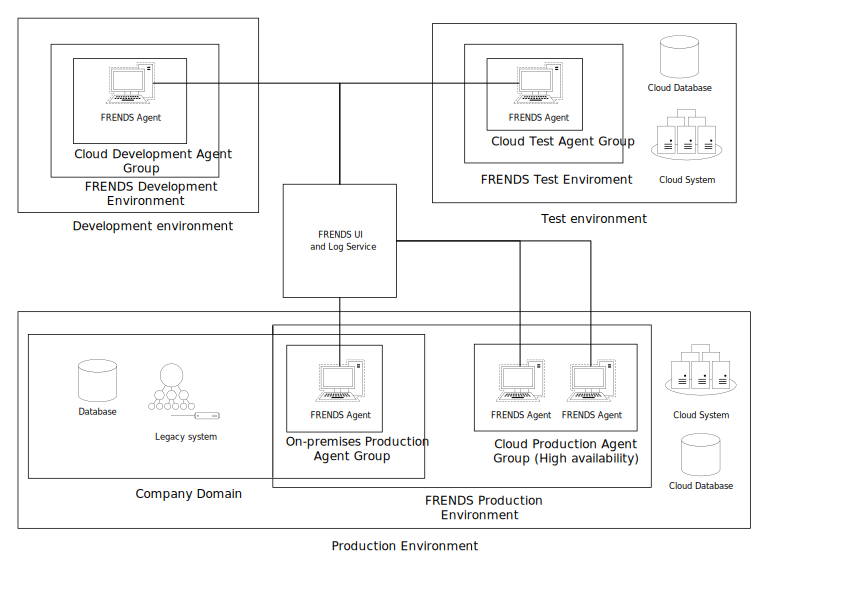
\includegraphics[width=\textwidth]{pictures/frends/FRENDS_Architecture.png}
  \caption{FRENDS architecture with five agents. The figure illustrates the possibility of FRENDS installation where the customer has one development, one testing, and three production agents. This customer has an on-premises production environment, where one FRENDS agent has been deployed. The production environment has also two FRENDS agent in the cloud. These two agents are in the same agent group, and they are configured to work in high availability mode to share the load.}
  \label{fig:Frends_architechture}
\end{figure}

\subsection{Process}
\label{sec:process}
Processes are how the orchestration layer is built in FRENDS. Each process defines an integration flow. They can be loosely coupled to other systems, so they form a miniservices. The miniservices are discussed in more detail in Chapter~\ref{sec:methods_of_integration}. The process consists of different elements, such as tasks and triggers. Processes are compiled as executable dynamic-link libraries (DLLs) and distributed to agents as NuGet packages~\cite{microsoft2018nuget}. Each process is versioned and may be deployed to multiple environments and agent groups.

Each process starts with at least one trigger and ends in a return element. The process can also have control elements, such as conditions for each loop, subprocesses, and error handlers. Figure~\ref{fig:Simple_process2} illustrates a process. 

A single execution of a process is called a process instance. Both process and process instance can be viewed through the FRENDS UI. Process instance contains all information related to a specific run of the process used to monitor and audit process runs. There are two kinds of processes available in FRENDS: regular processes (called processes) and subprocesses. Subprocesses are discussed in Section~\ref{sec:subprocess}. Processes are used to create integration orchestration or integration flows. They also visually document the process.

\begin{figure}[htb]
  \centering
      \includegraphics[width=\textwidth]{pictures/frends/Simple_process2.png}
  \caption{Screenshot of a process from FRENDS UI. This process starts daily at 1 a.m. or whenever manually initiate. It will read customer data from the database and then send invoices to each customer. In addition, the process can detect error happened during reading the database.}
  \label{fig:Simple_process2}
\end{figure}

\subsection{Subprocess}
\label{sec:subprocess}
A subprocess is used when different processes need the same functionality, such as error reporting, which is more complex than a single task. In other words, they also create reusable miniservices. Subprocesses can form a hierarchy where the FRENDS process executes a subprocess, which executes another subprocess, and so on. In this way, a process and subprocesses can form an integration orchestration layer where access to different systems is isolated in different subsystems. 

Example of the Subprocess hierarchy:
\begin{verbatim}
Main Process
  Subprocess
    Subprocess
      Subprocess
  Subprocess
Main Process
\end{verbatim}

In addition, the subprocess can be executed on a different agent group, in the same environment, then calling the process or subprocess. This way, parts of the process can be on different physical or logical locations. This enables the hybrid capabilities of FRENDS. For example, a process running on a cloud agent can call a subprocess on an on-premises agent. A process can have a subprocess attached that is called when the process is in error. They can be used to report or log unexpected errors.

The subprocess can also act as a conditional trigger. They enable using complex logic to be the condition when the process is executed. The conditional trigger is executed on the configured interval, and depending on the outcome of the subprocess, the parent process is either executed or not.

\subsection{Triggers}
Triggers define when a process should be executed. Triggers act as a starting point for the process and the first step in the process. They are started based on an event that the agent can receive or on a condition given by a conditional trigger. These events include a web service call received by the agent, a file being created, a message appearing in the queue, and a schedule activated within a time window. Triggers are the first element in the process editor canvas, and the process can have multiple triggers. Only web and file triggers provide some information about the location or path where the process is started. Other triggers, such as schedule or queue triggers, do not provide information about integration locations. Web triggers start processes after they receive Hyper Text Transfer Protocol (HTTP) or Hyper Text Transfer Protocol Secure (HTTPS) requests. Each HTTP trigger has a unique URL. File triggers start the process when a file matching the file filter is saved to the defined directory. 

\subsection{Tasks}
\label{sec:tasks}
Tasks are the building blocks of FRENDS processes. For example, a task could read a file or write something to a database. They are reusable components and have parameters that can be configured in the FRENDS UI. Configuring can be, for example, giving the file name and directory location to a task that reads files. Technically, a task is a class library targeting either the .NET Standard or .NET Framework. Most FRENDS tasks are open source, and the code is available via GitHub~\cite{community2018}~\cite{hiq2018frendstasks}.

\begin{figure}[htb]
  \centering
      \includegraphics[width=\textwidth]{pictures/frends/Process_run.png}
  \caption{Screenshot of a process execution from FRENDS UI. Executed task are colored with green, marking the path of executed integration flow.}
  \label{fig:Process_run}
\end{figure}

Figure~\ref{fig:Process_run} illustrates a successful process run, where the process execution path and task that have been run successfully have been highlighted in green. As seen in the figure, not all tasks are executed. In addition, the operator could click on any task and see the execution time, depending on the logging setting, and possibly see the task input and return values as well.

\subsection{Parameters}
\label{sec:parameters}
A parameter editor is used to tell tasks and other shapes what they should do. Therefore, configuring parameters is the second most important item in a process after building the process model itself. The parameter editor is very versatile and features rich code and a text editor, and only the parts relevant to this thesis are presented. Parameters contain all the information of all process endpoints, either straight or via environment variables. Therefore, investigating them and the environment variables is the only step required to acquire information for analysis to perform architecture recovery.

Parameters contain text that depends on the situation, such as structured query language (SQL) queries, XML “files,” URLs, or anything else. Figure~\ref{fig:sql_parameters} shows the FRENDS subprocess that contains one task and configuration for that task. The task configuration is on the right side. The task is a SQL query and performs the query shown in the figure. It takes the connection string from the environment variable, and the reference \verb|#env.AdventureWorks.ConnectionString| is shown.  The connection string also contains a password needed to connect the database, and it is therefore not revealed anywhere in the UI or logged anywhere. However, it can be obtained from the database. Environment variables are discussed more in Section~\ref{sec:environment_variables}. The task performs the SQL query:

\begin{minipage}{\linewidth}
\begin{lstlisting}[language=Sql]
SELECT TOP 1 [ProductID]
    ,[Name]
    ,[ProductNumber]
    ,[StandardCost]
    ,[ListPrice]
    ,[ProductCategoryID]
    ,[ProductModelID]
    ,[SellStartDate]
    ,CONVERT(varchar(max),[ThumbNailPhoto],2) AS 
        ThumbnailPhoto
    ,[ThumbnailPhotoFileName]
  FROM [SalesLT].[Product]
\end{lstlisting}
\end{minipage}

\begin{figure}[htb]
  \centering
      \includegraphics[width=\textwidth]{pictures/frends/Adventureworks_SQL_Parameters.png}
  \caption{Screenshot of FRENDS UI while editing process that only executes SQL query. View for editing task parameters is open and it shows the SQL query that can be executed.}
  \label{fig:sql_parameters}
\end{figure}

FRENDS enables writing the C\# code right into the parameter editor. It can be inside handlebars \path{{{}}} or anywhere after the parameter field type is changed to the Expression mode. In addition, FRENDS enables writing multiple different references in Expression mode or inside the handlebars. References always start with a hashtag. These references include, for example, environment variables \path{#env.name} and variables \path{#var.name}. When the process is compiled to an executable DLL, FRENDS resolves all references. It is possible to combine text with expressions. For example, one could write the URL of a destination as follows:

\nopagebreak
\begin{center}
\path{https://www.{{#env.CustomerName}}.com/api/v1/petshop }.
\end{center}

Given that CustomerName contains the correct name of the customer, this would be a working URL. However, it is also possible to combine expressions so that they form meaningful addresses only at runtime. For example,

\nopagebreak
\begin{center}
\path{https://www.{{#env.CustomerName}}.com/api/{{#env.Petshop.ApiVersion}}/{{#var.ApiName}}}
\end{center}
contains environment variables and variables in such a way that they do not form a valid address unless all environment variables are evaluated. That would be possible, but in this thesis, it is not done because replicating FRENDS’s entire parameter expansion would have been tremendous work.

Figure~\ref{fig:sql_parameters} shows an example of the FRENDS UI while editing parameters. Here, subprocess consists only one task: an SQL query. The actual query, task name, and a connection string obtained via the environment variable are present on the right-hand side of the picture. The connection string contains information on how to connect the database to the query. 

\subsection{Agent}
The agent is responsible for executing the integration flows or processes. The agent does not rely on any other FRENDS component to function. Therefore, integration processes keep running, even if some other FRENDS components are offline. The agents are connected to other component databases through a service bus connection. Each agent is assigned to one agent group. 

\subsection{Agent Group}
Agent groups form a farm configuration. They share configurations and states. Agents can share the load with each other and take over the execution from a failed agent. In addition, multiple agents can co-work in an agent group to enable high availability of services by sharing the load.

The process is deployed to agent groups and then delivered to each agent in the agent group. A single environment can contain multiple agent groups (i.e., cloud and on-premises agent groups in production).

\subsection{Environments}
Environments isolate agents for logical containers that share different roles. Usually, at least three environments are present: development, testing, and production. Each environment has agent groups assigned to it. Each environment also has different environment variable values, monitoring settings, and other settings, such as log and security settings. Processes can only be created in the development environment. They can be then deployed to other environments. It is possible to deploy a process in some environment without any agents but running them requires at least one agent. 

\subsection{Environment Variables}
\label{sec:environment_variables}
Environment variables play a key role in storing configuration information. They store information that is attached to a specific environment. This information is often related to a system where the integration process is connected, such as addresses, usernames, and passwords. Environment variables are organized into three groups: key-value pairs, hierarchical groups, and lists. When information is needed in the integration process, it can be accessed by referring to the environment variable. The correct value for each environment is automatically fetched. These references can be an unlimited number, and if the value must be changed, it must be updated only once in the environment variables. 

\begin{figure}[htb]
  \centering
      \includegraphics[width=\textwidth]{pictures/frends/Adventureworks_Env_Parameters.png}
  \caption{Screensot of FRENDS UI showing the environment variable editing view. The “ConditionalTrigger” group has four fields with their values set in the development environment.}
  \label{fig:env_parameters_editor}
\end{figure}

Environment variables can be accessed in a process by references starting with \verb|#env|. For example, in Figure~\ref{fig:sql_parameters}, the connection string is taken from the environment variable via the reference \verb|#env.AdventureWorks.ConnectionString|. Figure~\ref{fig:env_parameters_editor} shows the editing view of the environment variables. For example, \linebreak \verb|#env.ConditionalTrigger.SftpUsername| is set to have value \verb|demo| in the development environment.


\subsection{Log Service}
The log service handles all messages coming from agents and evaluate monitoring rules. Messages include heartbeats and log messages. The log Service also handles cleaning up the database by removing old process instances. Process execution status updates are sent to a management UI website by the log service.

FRENDS can log process execution information. Depending on the setting, anything from everything to nothing can be logged (e.g., only errors).

\subsection{Database}
FRENDS stores everything to its SQL database. Two databases are particularly interesting for this work: FRENDSConfigurationStore and FRENDSLogStore. \linebreak FRENDSConfigurationStore contains all process and their editing history. \linebreak FRENDSLogStore contains information about the process instances. By default, any instances older than 60 days are removed to prevent the database from growing too large. Therefore, data in FRENDS does not contain data for an extended period about how processes have been run. This limits the possibilities for what kind of traffic analysis would be possible.

\subsection{Traffic Analysis}
\label{sec:traffic_analysis}
The limitation of the possibilities of traffic analysis is that, currently, only process-level logs are available. It is possible to extract a task-level analysis from them, but not how much traffic goes to that system. Previously, process- and task-level traffic analyses have been made by Power BI in HiQ, but higher-level analysis first requires information on which processes connect to the same system. The work in this thesis can provide that information. However, the actual implementation of traffic analysis on the system level is out of the scope of this thesis.

\clearpage
\section{Expected Characteristics of Integration Architecture}
\label{sec:methods_of_integration}
In this chapter, it is first discussed how the chosen method of integration influences the architecture of the orchestration layer. If the chosen method is followed, it defines how different systems are connected. Then more general principles of network tools and their applications to orchestration architecture are discussed.

\subsection{Spaghetti Integration}
The simplest way to integrate systems is to connect them directly connect them. From the perspective of one system, all connections seem like a star. However, when all systems are presented, the connections look like spaghetti, hence the name. Spaghetti integration is illustrated in Figure~\ref{fig:spaghetti}. Star integration is also called point-to-point integration, as integrations are done from one point directly to another. The overall complexity of the spaghetti integration is not too high for a small enterprise, which has only a few systems. However, large and medium-sized enterprises have tens or hundreds of different systems. Therefore, the different point-to-point connections become unmanageable when old systems are replaced, or new systems are added~\cite{josuttis2007soa}. Unexpected dependencies will become too common. 

\begin{figure}[htb]
  \centering
      \includegraphics[width=\textwidth]{pictures/Architecture/Integraatiospagetti.png}
  \caption{When an enterprise has only a small number of systems, the spaghetti integration remains a viable option. As the number of systems grows, the integrations start to look like a plate of spaghetti. The figure illustrated connections between 20 different systems, divided into four different network locations. In real life, there are usually even more connections, and therefore real-life diagrams are a lot messier.}
  \label{fig:spaghetti}
\end{figure}

Usually, heterogeneous or proprietary interfaces raise the cost of spaghetti integration, but real difficulty comes from the fact that the time and cost to add new subsystems increases exponentially. Therefore, medium-sized enterprises often start seeing the rising cost of integrations and start looking for alternatives to spaghetti integration~\cite{josuttis2007soa}.

\subsection{Hub and Spoke Integration}
Difficulties with spaghetti integration architecture were first addressed by the hub and spoke systems. They replace spaghetti integration by creating a single system, called a broker, where all other systems were directly connected. The broker allows loosening the coupling between systems by indirect asynchronous communication. The sender does not need to wait for a response but instead could continue its execution after sending the message. In addition, the sender would not need to know the destination of the message.

However, the broker would quickly become a bottleneck and a place of single-point failure. In addition, as it a single destination for messages, it is difficult to scale this model across multiple geographical locations. Moreover, the broker is often supporting only a specific vendor’s technology. The support for all kinds of technologies (often legacy) is problematic. Nowadays, the broker model is not generally used due to the advantages of newer approaches~\cite{mulesoft2018understanding}.

\subsection{Service Oriented Architecture and Macroservices}
\label{sec:service_oriented_architecture_and_macroservices}
The Service Oriented Architecture (SOA) was designed to hide different systems with different capabilities and publish them as a general-purpose business service. Hence, services created in one project were available in the following projects, which would reduce the overall costs. For example, a subscription service or customer information service could be one service in SOA. The SOA architecture is usually built on top of the Enterprise Service Bus (ESB)~\cite{josuttis2007soa}.

ESB illustrated in Figure~\ref{fig:esb} is a specialized subsystem designed to enable communicating between other systems. It connects horizontally to other systems. Horizontal integration means communication between different systems supporting different functional areas of a business. ESB was developed to make it possible to connect various services and thus enabling SOA as a design principle; multiple services could be connected via one bus.

\begin{figure}[htb]
  \centering
      \includegraphics[scale=0.7]{pictures/Architecture/ESB.png}
  \caption{Enterprise Service Bus (ESB). ESB connects multiple different services via one bus, resulting very simple architecture.}
  \label{fig:esb}
\end{figure}

\begin{figure}[htbp]
  \centering
      \includegraphics[width=\textwidth]{pictures/Architecture/Macroservices.png}
  \caption{Illustration of a business process connecting to external systems using a service layer (usually an ESB). All connections from integration go to the same destination, that will direct them to the correct systems. Systems are large monolithic services, and therefore they are described as a macroservices. }
  \label{fig:macroservices}
\end{figure}

Granularity (i.e., the size of the published service) of services following SOA architecture was high; therefore, these are also called macroservices. The problem with macroservices is the pursuit of generality, and their monolithic nature drives the development costs too high. In addition, when business operations change, the cost of changing macroservices is usually high. A business process using macroservices is illustrated in Figure~\ref{fig:macroservices}. Granularity is illustrated in Figures~\ref{fig:macroservices},~\ref{fig:microservices} and~\ref{fig:miniservices}. The first one describes macroservices, the second is microservices, and the third is miniservices used by a business process. 

\subsection{Microservices}
The microservice architecture was developed to address problems in macroservices. They were developed as a small and independent component. They could be deployed to production without any dependencies on other components or systems. Microservices are technology agnostic, so they do not require any specific technology. That design also provides their ability to scale exceptionally well, and they are used in the largest web services. A business process using microservices is illustrated in Figure~\ref{fig:microservices}.

\begin{figure}[htbp]
  \centering
      \includegraphics[width=\textwidth]{pictures/Architecture/Microservices.png}
  \caption{Illustration of a business process connecting to external systems that are implemented as a microservices. Systems are small and individual, and they perform only one thing so that they might call other systems as well.}
  \label{fig:microservices}
\end{figure}

Microservices also contains many aspects that are disruptive to any enterprise~\cite{balalaie2016microservices}. One of the toughest is that each microservice owns its own data. This comes from the fact that the microservice cannot have any dependencies anywhere. Therefore, the microservice cannot rely on data in the enterprise resource planning (ERP) or customer relations management (CRM) systems. Therefore, microservice development and usage require a massive change in the old way of thinking about business processes and developing systems. This independence is a crucial differentiator between microservices and spaghetti integration. In spaghetti integration, everything has dependencies everywhere, whereas no dependencies exist in microservices. 

\subsection{Miniservices}
\label{sec:miniservices}
To address problems in both macroservices and microservices, miniservices were developed. Miniservices try to incorporate the best aspects of both. They differ from microservices in that they can be loosely coupled to other services. Miniservices are easily deployed to production, but even loose dependencies to external systems can form a limitation to scaling. Dependent systems might not scale well. A business process using miniservices is illustrated in Figure~\ref{fig:miniservices}.

\begin{figure}[htbp]
  \centering
      \includegraphics[width=\textwidth]{pictures/Architecture/Miniservices.png}
  \caption{Illustration of a business process connecting to external systems that are implemented as a miniservices. Systems are not as small as in microservices, and they might depend on other systems, but also call them when necessary.}
  \label{fig:miniservices}
\end{figure}

\subsection{Macroservices, Miniservices, and Microservices from the Architectural Viewpoint}
\label{sec:macro,mini,and_microservices_from_architectural_viewpoint}
Whether systems use macroservices, miniservices, or microservices as the designing principle has a significant effect. Macroservice appears as one system regardless of how many operations can be performed, whereas each micro part in a microservice appears as one system. As described in Section~\ref{sec:enterprise_application_integration}, integration occurs between multiple systems that do not share the same architectural principles. Therefore, the recovered architecture might contain an aspect of multiple methods of integration.

As discussed in Sections~\ref{sec:process} and~\ref{sec:subprocess}, FRENDS processes, and subprocesses can be viewed as a miniservice. Therefore, most integrations should look like the spaghetti integration illustrated in Figure~\ref{fig:spaghetti}. The crucial difference between the spaghetti integration and microservices and miniservices is that, in spaghetti integration, the integrations are not implemented using any particular system, such as an EAI platform. The EAI provides multiple benefits, like governing the monitoring and reusability of components, regardless of the architecture used. These are discussed in more detail in Section~\ref{sec:enterprise_application_integration}.

\subsection{Centrality Measures}
As discussed in Section~\ref{sec:software_architecture_archaeology_in_general}, orchestration architecture can be represented as a network. Therefore, the normally used methods to study networks can be applied to orchestration architecture. Usually, centrality measures, such as betweenness, closeness, and page rank, are used to study the importance of different nodes in the network.

However, they are not important in this network because different integration flows are usually separate. The processes can use the same data, for example, one process might involve customer creation, and another can also use that information. Other than handling the same data, the processes do not have a relationship; for example, it is very unusual for a process to depend on another process because it would be a poor design. Subprocesses would be a more viable option. Furthermore, the fact that integration flows are usually separated prevents errors spreading in the network.

\subsection{Clustering}
\label{sec:clustering}
Clustering is a technique to detect higher level organization in networks. Networks are said to have a cluster, also known as a community if a network can be grouped by node groups so that each group is more densely connected internally than to other groups. Multiple strategies to form clusters exist and some of them allow overlapping communities. Usually, clusters are detected from this type of network using the stochastic block model or modularity optimization.

The stochastic block model is widely used to detect clusters~\cite{abbe2015community}. It would be a useful tool in solving this kind of problem; however, it was agreed with the customer that their data would not leave the environment. Installing tools such as the graph-tool (a Python module)~\cite{peixoto2014graph} would have required installing software that was not possible due to the policy limits.

Not being able to use the stochastic block model leaves the modularity measure as a viable option to detect clusters. The modularity method measures the number of edges within the cluster subtracted from the expected number of edges calculated from a random network. The clusters themselves can be found through modularity optimization. For that, the algorithm presented in~\cite{blondel2008fast} was used.

\subsection{Multipartite Network}
\label{sec:multipartite_network}

At first, the network appears as a multipartite network. However, closer examination shows that this is not the case. Similar methods could nevertheless reveal useful information about the network structure. A $k$-partite network has $k$ kinds of vertices, and connections are only allowed between different kinds. When $k = 2$, this is called a bipartite network, and when $k = 3$, it is a tripartite network.

This network is partitioned as follows: Data is written or retrieved in the endpoints. Connections can be made between endpoints and processes and between endpoints and subprocesses. Processes can have connections to both endpoints and subprocesses. A major point here is that, in addition to processes and endpoints, subprocesses can have links to other subprocesses. In multipartite networks, nodes are only allowed to have connections to different kinds of nodes. If this were a multipartite network, a subprocess would not be able to connect to another subprocess.

Although the network is not a true multipartite network, it is possible to remove endpoint nodes and then make a new link between the remaining nodes if at least one common neighboring endpoint node exists in the original network. Likewise, processes and subprocesses can be removed, leaving only endpoint nodes. New links are added between endpoint nodes if they could be connected in the original network by any number of processes or subprocesses. Because of formed network resemble unipartite networks markedly, terms \textit{unipartite} is used to describe networks and term \textit{multipartite} to describe the original network. 

The result is two different networks: one with only processes and subprocesses that shows how they are connected and another with endpoint nodes that show how they are connected. The first network should clearly show whether different environments are separate and thus even show separate networks for each environment. In theory, the second network could reveal the architecture of the systems connected to EAI, as the EAI platform itself is completely abstracted away.


\subsection{Scale-free Networks}
\label{sec:scale_free_networks}
Usually, integration orchestrations are separated into three separate environments: development, testing, and production. They should not contain any connection to each other as production should not depend on testing environments that do not have sufficient monitoring, for example. Otherwise, the network might be a small-world network. A topology of the network can be tested by calculating connected components, node degree distribution, and a few other metrics. 

Scale-free networks, or scale-free graphs as they are often called, are formed in the dynamic process. Scale-free networks are known to arise from notably different phenomena.They form when new nodes are added to the network, forming new connections. If the probability of a node connecting to a new node depends on the old node connections, a scale-free network will emerge.  This leads to the phenomenon of the “rich get richer,” and the nodes with the most links will get even more of them. Most real-world networks develop over time. Thus, scale-free networks are found in various real-life scenarios~\cite{buchanan2002nexus}.

\clearpage
\section{Methodology}
\label{sec:methodology}

This chapter discusses how integration strategies discussed in Section~\ref{sec:integration_strategies} use different technical methods to connect to external systems. In addition, those methods are exploited to recover architecture from the integrations implemented on FRENDS.

The three main ways to represent external systems are paths, URIs, and connection strings. A combination of these is common; for example, SFTP file sharing combines paths and URLs. Various integration strategies use these to connect to external systems, but the details vary.

\subsection{Databases}
Connection strings specify how to connect to the data source. They are usually used to connect databases or other data sources, such as spreadsheets. The two most-used database languages used in corporations are Microsoft’s T-SQL and Oracle’s PL/SQL that both extends SQL. Their connection strings share a common characteristic, where parts of the connection string are separated with a semicolon (“;”) and the parts themselves contain a keyword and value~\cite{microsoft2018connection}~\cite{oracle2018connecting}. Databases contain multiple tables containing different data relating to different items. In this work, which table integration process writes the data is not investigated. The whole database is treated as one system and thus, one architectural component.

\subsection{File Transfer}
File transfer moves files between locations, as the name suggests. Fully qualified paths or absolute paths describe a location of a file or web resources starting from a file system root, drive letter, or full domain~\cite{microsoft2018naming}. Relative paths contain only part of the absolute path. Thus, relative paths usually locate resources relative to the current location. 

\subsubsection{Uniform Naming Convention for paths}
The Uniform Naming Convention (UNC) is a standard method in Windows to describe the location of a file, directory, or printer. The simplified generic form for remote resources is \path{\\ComputerName\SharedFolder\Resource}. Local files usually start with the drive letter \path{C:\\Folder\File}~\cite{microsoft2018naming}. Relative paths do not start from a computer name or drive letter but from the “middle” of the path, for example, \path{SharedFolder\Resource}.

\subsubsection{Unix-style file system paths}
Paths in portable operating system interface (POSIX) systems~\cite{ieee2018definitions} or Unix-like systems, for example Linux, use notation that is generic for \path{hostname:/Directory/Resource} for the remote location and \path{/Directory/Resource} for the local. The leading slash (“/”) marks the root directory (i.e., the beginning of the file system hierarchy). Paths can also be relative, and then they do not start from the root but from the middle of the path, for example, \path{Subdirectory/Resource}.  

\subsubsection{File shares}
It is possible to share any directory to be available in the network. The technical details on how sharing works varies between Windows and Unix-like systems, but the general principles are the same. It is also possible to give a new address (i.e., a path to access a shared directory remotely). For example, using the UNC convention, a resource in a local location can be found as follows:

\begin{center}
    \path{D:\EAI\FileStorage\ERP\Invoices\Company AB.\VacationFiles\Temporary Storage\Incoming files\ },
\end{center}
and could be shared at location
\begin{center}
    \path{\\Servershare01\Company AB.\VacationFiles\in\ }.
\end{center}

It is also possible to share the same directory or resource multiple times with different paths. For example, it is possible to share a local location:
\begin{center}
    \path{D:\EAI\FileStorage\ERP\ }
\end{center} as \path{\\ErpFiles\ }, thus enabling access to a previously shared location via the path:
\begin{center}
    \path{\\ErpFiles\Invoices\Company AB.\VacationFiles\Temporary Storage\Incoming files\ }.
\end{center}
From that location, it is impossible to know the underlying hierarchy.  Now, it is hard, or even impossible to determine without further knowledge whether these two shared locations lead to the same place or not. Therefore, it is impossible to recover such architecture without additional knowledge.

\subsection{Messaging: Internet-based Strategies}

Correct URLs have a strict format~\cite{hoffman2005telnet} and represent the location and access method of some resources on the internet. Moreover, URLs support only American standard code for information interchange (ASCII) characters, but that can be extended by canonicalization~\cite{microsoft2018handling}. Canonicalization enables encoding of a non-ASCII character with ASCII characters. Usually, a URL is not written completely and therefore, is not “correct.” One commonly known example is the use of the WWW, World Wide Web prefix in a URL~\cite{bernerslee1994uniform}, as is in \path{www.example.com} where \path{http://} is omitted, for example. Another notable addition is the Uniform Resource Identifier (URI) is a file URI~\cite{kervin2017file} used to locate files on the internet. In general, it is tricky to detect all URI-like strings, but fortunately, it is not necessary because they are usually hierarchical locations and detecting that hierarchy is sufficient, as discussed more in Section~\ref{sec:matching_with_regex}.

\subsection{Messaging: Buses and Queues}
\label{sec:messaging_buses_and_queues}
As described earlier, there are two ways to deliver messages: either by bus, such as the Azure Service Bus or by queue, such as AMQP. Both work the same way in that all messages are sent to one place regardless of where they are going or what they contain. Therefore, it is significantly more challenging to identify the message destination from the integration process implementation. Additionally, identifying the destination of messages sometimes requires information on a system that has a subscribed message from a bus or queue, and therefore, knowing the destination from the implementation of the integration process is sometimes impossible. There might be multiple queues that could be identified but only one bus, and information that the integration process is connected to the bus is not very informative. Therefore, buses are left out of architecture recovery.

At the time of writing this thesis, FRENDS has only limited support to AMQP queues. Messages can be only read from it, and no support exists for other queues. Therefore, integrations that use queues are not made, and these are left out of the architecture recovery.

\subsection{Matching with Regex}
\label{sec:matching_with_regex}
Paths, URLs, and others are well-structured strings, so it makes sense to use a regular expression, regex, to match them. Regex is a widely used language to find patterns, such as URLs or paths, in the text. In this work, the regex processor called Perl Compatible Regular Expressions~\cite{pcre2018pcre} (PCRE) was used. It provides a robust and well-documented environment to execute regex.

A significant difficulty in using regex comes from the fact that different systems use different characters with special meanings. For example, if delimiters are present in data, they must be escaped with escape characters to avoid delimiter collision. Usually, backslashes (“\textbackslash”) are used as escape characters. The problem arises when different systems use the same characters as delimiters, and the information goes through multiple systems. Each system adds escape characters that the next system needs to escape. Therefore, the massive number of backslashes needed for escape characters makes the regex patterns nearly unreadable. This phenomenon is known as “the Backslash Plague” or “leaning toothpick syndrome”~\cite{perlintro2018perldoc}. For example, to match \path{//} after the protocol part of the URL, each forward slash is escaped with a backward slash (\path{\/}). Moreover, when doubled, as in URLs, this becomes \path{\/\/}.

We consider a similar problem with UNC by example. In UNC, paths might begin with double backward slashes \path{\\}. Both might be escaped by the external system, resulting in four backslashes \path{\\\\}. Therefore, the regex matching two backward slashes requires eight backslashes \path{\\\\\\\\}. Besides that, the backward slashes might have to be escaped twice in UNC, and the UNC might also start with a drive letter followed by a backward slash and colon \path{\:}. Therefore, the regex matching the start of the UNC path is \path{[a-zA-Z]:\\{1,2}|\\{2,4}}. The previous regex matches any string that starts with an ASCII letter followed by a colon and one or two backward slashes, or a string that starts with two to four backward slashes. The regex also matches a string starting with three backward slashes, but generally, they are not presented in the data and can easily be filtered out afterward.

\subsection{False Positives}
\label{sec:false_positives}
Integration processes can and often do contain a vast number of URLs and file paths that do not represent external systems. These include XML schema locations and the locations of temporary files. They are false positives as they do not represent the location of an actual place where data is written or where the data is read. They have to be filtered out, or otherwise, clustering, discussed in section~\ref{sec:clustering}, would recognize false positives, such as a temporary file, as an individual system. 

False positives are, however, easy to filter out because XML schema locations are prefixed with “xmlns.” File paths to local resources can be identified because, at the time of writing this thesis, FRENDS only runs on Windows, where the drive letters C, D, and F are used for the local file system. FRENDS references, or parts of them, might also be detected as URLs under certain circumstances. For example, the environment variable \verb|#env.customerAddress.fi| is roughly like the URL \path{customerAddress.fi}. FRENDS references will always start with either \verb|#var|, \verb|#env|, \verb|#process|, or \verb|#result|, so they are easy to filter out.

\subsection{Hierarchical Clustering}
\label{hierarchical_clustering}
A common characteristic of paths and URLs is that they provide information about the underlying organization by design. They are designed to tell the hierarchy that starts somewhere and leads somewhere. For example, UNC starts from a drive letter, followed by folders. As more folders are added, the location becomes more specific. Therefore, removing folders from the end enables one to move upwards in the hierarchy, thus enabling the clustering of larger units. 
For example, the path
\begin{center}
    \path{D:\EAI\FileStorage\ERP\Invoices\Company AB.\VacationFiles\Temporary Storage\Incoming files\ }
\end{center}
could be reduced to 
\begin{center}
    \path{D:\EAI\FileStorage\ERP\Invoices\Company AB.\ }
\end{center}
and, alternatively, even to
\begin{center}
    \path{D:\EAI\FileStorage\ERP\ }.
\end{center}

The former would represent all file paths to Company AB and, later, all ERP connections. The URL works is a similar fashion. For example, the URL 
\begin{center}
    \path{http://www.example.com/api/v1/Petshop/store/order/}
\end{center}
could be split to 
\begin{center}
    \path{http://www.example.com/api/v1/Petshop/ }.
\end{center}

The removal of levels of the hierarchies is an essential part of how clustering would be performed, as otherwise multiple very similar paths would represent individual unrelated connections. The available literature did not contain any insight into this problem. Moreover, the author did not produce any smart algorithm to determine the number of levels removed, so it was left as manually configurable. 

The hierarchical clustering was done before the network was constructed. Therefore clustering technique Modularity Optimization, discussed in Section~\ref{sec:clustering} were applied to the network that was already clustered with the hierarchical clustering. This two-phase approach to clustering resulted in much better results than either technique alone.

\clearpage
\section{Power Bi Model and other implemented software}
\label{sec:powerbi_model_and_r}
This section provides a simplified description of the implemented Power BI model and other tools. The work is done on the Power BI~\cite{microsoft2018power} with the Network Navigator Chart add-on~\cite{microsoft2018network} to create an illustration from the networks. Additionally, the R~\cite{r2018language} with the rjson package~\cite{alex2014rjson} was used inside Power BI and to generate more illustrations. In addition, Gephi~\cite{bastian2004gephi} was utilized to produce illustrations of the networks.

Unfortunately, the Power BI model with the R code cannot be published due to concerns regarding the accidental release of customer data and business operations. It was necessary to enable native database queries in Power BI, and the database must be marked as public to make it possible to run R scripts on the data obtained from the SQL database. Effectively, it would disable all privacy and data protections inside Power BI. It must be done because Power BI cannot protect data because the data are handled with the R code, which could theoretically do anything. The R language was used because Power BI does not support regex or similar technologies for pattern matching. Rest of this chapter describes what was needed to form network representation of the orchestration layer in addition to things described in Chapter~\ref{sec:methodology}. 

\subsection{Process versions and colors}
\label{sec:processes_versions_and_colors}
In the database table \verb|PROCESS_VERSION|, each process that is deployed is listed. It also contains information on which agent group and the environment the processes are deployed. Because that information is used multiple times, it is read in its own table and processed in Power BI only once. After that, each process is attached to a color based on its environment that is used to make networks. Example data after transformations (for clarity the process ids are truncated):

\nopagebreak
\verb=ID   PROCESS_ID VERSION  ENVIRONMENT  AGENT_GROUP  Color=

\nopagebreak
\verb=466  825...86F  22       Default      Default      Red=

\nopagebreak
\verb=438  19A...FA1  3        Prod         Prod         Green=

\subsection{Process names} 
Usually, a process has the same name in each environment. However, when all processes from all environments are plotted in the same network, it is inconvenient if there are, for example, three processes plotted with the same name. Therefore, the environment name is added in front of process name (e.g., \path{Prod | Example Process Name} and \path{Test | Example Process Name}). It is done by expanding information obtained in~\ref{sec:processes_versions_and_colors} by adding the process name and a similar environment. In addition, the Process ID is attached to the environment because it is necessary to differentiate the processes when they are deployed to different environments. Example data after transformations:

\nopagebreak
\verb=NameAndAG                        IDandAgentGroup  Deployment.Color=

\nopagebreak
\verb=Prod | GO: It is network  (2)    13823Prod        Green=

\nopagebreak
\verb=Default | GO: It is network  (2) 13823Default     Red=

\subsection{Environment variable processing}
\label{sec:environment_variables_processing}
First, environment variables are read from the database and unnecessary columns, such as old versions of environment variables, are filtered out. The R script is then used to process the JSON, where the environment variables are stored. The script reconstructs the environment variables in the same format as they are written in the Parameter Editor (e.g., \verb|#env.Customer.Name|). In addition, the R script searches the connection endpoints as described in Section~\ref{sec:matching_with_regex}. Environment variable names are then combined with values from the R script. Then, the empty environment variable values and other artifacts, discussed in Section~\ref{sec:false_positives}, are filtered out. Finally, the right environment is placed in the place of \#env, so it becomes possible to differentiate the environment variable names between environments. For example, \verb|#env.Customer.Name| is changed to \verb|#Test.Customer.Name| or \verb|#Production.Customer.Name|. It is done because environment variables have different values in each environment. After the change, each environment value name points only to one value. Example data after transformations (for clarity the unique ids are truncated):

\nopagebreak
\verb=ID    UNIQUE_ID    EnvValue                EnvName=

\nopagebreak
\verb=1137  ADF...6FE    f:\\kuuukko\pics.jpg    #Test.GO_network.path=

\nopagebreak
\verb=1137  ADF...6FE    example2.com            #Test.GO_network.url=

\subsection{Subprocess Trouble}
\label{sec:ubprocess_troubles}
Subprocesses stored in the FRENDS database are like normal processes but differ on a few points. For example, they use slightly different escaping methods for special charters. Additionally, subprocess can call subprocesses from normal processes or subprocesses. Therefore, subprocesses are handled aside from normal processes. First, subprocess information is read from the database. Then, old subprocesses are filtered out, and the description field of the subprocess is cleaned. The R script is used to determine which subprocesses the process is calling. Then, the result from R is cleaned and modified to the Power BI list. The environment name is added to the process id as well as the process name. An R script is used to search the connection endpoints, as described in Section~\ref{sec:matching_with_regex}.

The Network Navigator and a few other network tools cannot make the connection between two source nodes. Therefore, the subprocess call has to represent an additional node between the process and subprocess. In the database, FRENDS stores only reference in the process, indicating it calls the subprocess, but not another way around. An R script is run to make a connection between the subprocess and the process that called it. Example data after transformations (for clarity unique ids and names are truncated):

\nopagebreak
\verb=IS_SUBPROCESS NameAndAG          UNIQUE_ID VERSION IDandAgentGroup=

\nopagebreak
\verb=False         Default | test...  4CC...A67 15      2546Default=

\nopagebreak
\verb=False         Prod | GO: It ...  597...253 2       13823Prod=

Moreover, FRENDS saves only a connection from the calling process to a called one, not the other way around. Thus, it must be determined with an R script.

\subsection{Processes}
\label{sec:processes}
In addition to process information, all other information from other steps is merged into the process information to obtain the complete node-edge list. It is done together with the processing process information to avoid the receptive steps in the Power BI model. First, the process information is loaded from the database. Then, the information from Section~\ref{sec:processes_versions_and_colors} is merged.  The old processes are filtered out, and unnecessary columns are cleaned. An R script is run to detect URLs, UNC, and other paths as described in Section~\ref{sec:matching_with_regex}. Environment information is then merged into the Process ID and environment variable name (i.e., \verb|#Production.Customer.Name|). Then, the information about the environment variables and their values are obtained from Section~\ref{sec:environment_variables_processing}. 

Using environment variables in the process and their corresponding values in each environment, it is now possible to combine the information and obtain an endpoint for each process stored in the environment variables. The following step is to combine the subprocess as endpoints and the reverse subprocess connection that was generated in Section~\ref{sec:ubprocess_troubles}, so the connection from the subprocess to the process was formed as well. After that, multiple delimiters, characters, and other items must be filtered out, and the endpoints are clustered as described in Section~\ref{hierarchical_clustering}, preserving only the first four levels in the path. It was manually tested to prove the most satisfactory results. However, some paths would still require stricter cutting, but it would lead other paths to be cut too aggressively. 

\subsection{Generating networks}
After everything is processed in Power BI, in Section~\ref{sec:processes}, a complete list of edges is available. The Network Navigator is used to generate an interactive visualization of the network. Its biggest downside is that it does not support showing a large number of nodes, so it cannot show all the environments at the same time. However, all nodes can be plotted with Gephi. These networks are discussed in Chapter~\ref{sec:analysis}. Figure~\ref{fig:ExampleNetwork} shows an example of the visualization of the network. Color of process and subprocess nodes show their environment. Endpoint nodes of different connections are in gray.

\begin{figure}[htb]
  \centering
      \includegraphics[width=\textwidth]{pictures/network/GS_verkosto_lahikuva.png}
  \caption{Colored circles are processes on different environments; gray circles are endpoints. Nodes are in force-directed layout and they were allowed to overlap. The figure is a screenshot from Network Navigator.}
  \label{fig:ExampleNetwork}
\end{figure}

\clearpage

\section{Analysis}
\label{sec:analysis}
The main aim of this thesis was to determine how software can automatically recover orchestration architecture from the implemented integrations. Two different aspects are required to make architecture recovery feasible. The orchestration layer on the EAI platform must be parameterized, and integration flows must follow a microservice or miniservice paradigm as the design choice. Parameters only contain a small portion of code, while still containing all the necessary information, so they make this task practical. This is discussed in more detail in Section~\ref{sec:parameters}. The microservice or miniservice as an architecture makes it possible to recover architecture. If all integrations were done in the same macrosystems, there would not be any architecture to be recovered at all. In addition, resulting architecture should look more or less like spaghetti, as FRENDS processes are miniservices. These are discussed in more detail in Section~\ref{sec:macro,mini,and_microservices_from_architectural_viewpoint}

\begin{figure}[htb]
  \centering
  \includegraphics[width=\textwidth]{pictures/network/AllNodesEnvColor.png}
  \caption{Illustration of a network constructed from the data that was used to test the recovery implementation. All nodes are in a force-directed layout. The colors represent the environment where each node belongs or indicate whether it is an endpoint. The division of these is intentionally left out. The nodes are allowed to overlap, and their labels are intentionally left out. One giant component and only a few small components exist. On the left side, one isolated component with only three process nodes and numerous endpoint nodes are shown. Endpoint nodes are repeatedly connected to process nodes from multiple environments.}
  \label{fig:AllNodesEnvColor}
\end{figure}

The orchestration architecture is then represented as a network to enable further analysis. However, for the customer whose data was used to test implementation, FRENDS is used to implement critical business processes. Thus, only the summary is shown. In addition, in many figures, the precise amounts or names are not given.

Figure~\ref{fig:AllNodesEnvColor} is an illustration of all the nodes in a network. The colors indicate whether a node is is an endpoint (i.e., a location where data are read or written) or a process and which environment it belongs. This figure illustrates the multiple key properties of the network. Most nodes are connected to each other and form a so-called giant component. The nodes are considered connected if there is some way to connect the nodes by links and other nodes. Only nodes that have a small number of links have been left out of the giant component. The only exception is three nodes that share a huge number of endpoints. They can be seen on the left-hand side of the network. A manual inspection of these processes reveals that they all share the same file backup location that uses a highly hierarchical folder structure, which hierarchical clustering was not able to shrink.

The figure clearly shows that most endpoints in the giant component have links to nodes from multiple environments. Thus, the production environment is not separate from the testing environment. However, due to a high number of nodes connection environments list of nodes connecting the environments did not prove to be valuable for this customer. Manual inspection of the network revealed that it presents the architecture of the integration orchestration is approximately correct. The developed method thus outperforms more general architecture recovery methods that are known for their poor performance. As discussed in Section~\ref{sec:clustering}, the researcher investigated whether modularity optimization could be used to detect business applications. The resulting groups are used to color nodes in Figure~\ref{fig:AllNodesModColor}. Clearly, modularity can identify groups within the giant component. Manual inspection revealed that they correspond to some degree the actual systems being used, but it was generally not able to detect different systems correctly.

\begin{figure}[htb]
  \centering
  \includegraphics[width=\textwidth]{pictures/network/AllNodesModColor.png}
  \caption{This is Figure~\ref{fig:AllNodesEnvColor}, but the colors are assigned to the 30 largest groups detected using modularity optimization. All nodes are in a force-directed layout. Nodes can overlap, and their labels are intentionally left out. Clearly modularity optimization can detect some structure from network, but detected groups did not corresponded to actual systems based on a manual inspection.}
  \label{fig:AllNodesModColor}
\end{figure}

\clearpage
\subsection{Multipartite Analysis}
As discussed in Section~\ref{sec:multipartite_network}, the network was divided into two parts. In the first part, all endpoint nodes were removed, and the neighbors of each removed node were connected to each other. In Figure~\ref{fig:UnipartiteEndpoints}, the endpoint nodes are preserved, and the process and subprocess nodes are removed in the unipartite projection. The structure is nearly absent in this network, as most nodes have only very simple connections to each other. Therefore it can not be used to detect systems as speculated in the Section~\ref{sec:multipartite_network}.

\begin{figure}[htb!]
  \centering
  \includegraphics[width=\textwidth]{pictures/network/UnipartiteEndpoints.png}
  \caption{A unipartite projection of a network shows connections between endpoint nodes in a force-directed layout. A color is assigned to all six groups found using modularity optimization. Nodes are allowed to overlap, and most nodes are collapsed to a few very tight groups. The node labels are intentionally left out. Clearly, this projection lacks most of the structure that was visible in the Figure~\ref{fig:AllNodesEnvColor}.}
  \label{fig:UnipartiteEndpoints}
\end{figure}

Figure~\ref{fig:UnipartiteProcessEnvColors} shows a unipartite projection, where process and subprocess nodes are preserved, and endpoint nodes are removed, and the neighbors of each removed node were connected to each other. The colors represent the environment where each node belongs. This network has a much clearer structure than the structure in Figure~\ref{fig:UnipartiteEndpoints}. However, it shows only how processes and subprocess are related to each other. Therefore, it can be used to group processes and subprocesses together. The original network would also provide this information easily. Clearly, nodes from different environments have multiple connections.

The degree and component distribution were also done with unipartite networks, but they did not provide any additional information. Therefore, in its entirety, the multipartite analysis did not provide new information.

\begin{figure}[htb]
  \centering
  \includegraphics[width=\textwidth]{pictures/network/UnipartiteProcessEnvColors.png}
  \caption{A unipartite projection of a network shows connections between process and subprocess nodes in a force-directed layout. The colors are the same as in Figure~\ref{fig:AllNodesEnvColor}. The nodes are allowed to overlap, and their labels are intentionally left out. Clearly this projection have much richer structure than that visible in Figure~\ref{fig:UnipartiteEndpoints}.}
  \label{fig:UnipartiteProcessEnvColors}
\end{figure}

\clearpage
\subsection{Degree and Component Distributions}
The degree of the node is the number of links the node has. The degree distribution is the probability distribution of different degrees that nodes have in a network. It is well known that, in scale-free networks, the degree distribution follows a power law. Thus, when plotted on a logarithmic scale, the degree distribution forms a line if the network is scale-free. Scale-free networks are discussed in more detail in section~\ref{sec:scale_free_networks}.

\begin{figure}[htbp]
  \centering
  \includegraphics[width=\textwidth]{pictures/network/DegreeDistribution.png}
  \caption{The degree distribution of every node in the network is shown. The axes are in logarithmic scale, and their labels are intentionally left out. The degree distribution for all nodes is shown with stars. Other points show the degree distribution for a subset of nodes (e.g., for the production environment). There seems to be a clear trend, but the points do not form a line; thus, the degree distribution does not follow a power law. In general, it seems that endpoint nodes have a higher ratio of high degree nodes than other nodes. There is no clear difference between development, testing, and production nodes.}
  \label{fig:degree_distributionWhole}
\end{figure}

In Figure~\ref{fig:degree_distributionWhole}, the degree distribution is presented for the whole network and each environment. The points do not form a line; that is a sign that degree distribution does not follow a line. The Kolmogorov–Smirnov test is utilized to test if degree distribution follows a power-law. Table~\ref{tab:degree_distribution} summarizes the results. It shows that the degree distribution does not follow a power law; thus, the network is not scale-free. Smaller values of D and p in the table indicates better fit~\cite{nepusz2019fitting}~\cite{newman2005power}~\cite{clauset2009power}. However, there are multiple nodes with a high degree that act as a hub in the network. The hubs are over-represented compared to a power-law: the network is more long-tailed (i.e., it has more high degree nodes) than a scale-free network. Manual inspection revealed that, for example, the backup location was among the nodes with highest degrees, giving a natural explanation to the high amount of links acquired by some nodes.

\begin{table}[htb]
\centering
\begin{tabular}{ l c r }
  Exponent & D & p \\
  \hline
  1.570712 & 0.15194 & 0.924982 \\
\end{tabular}
\caption{The Kolmogorov–Smirnov test results on the degree distribution show that the estimated exponent for a power law is roughly 1.57. The relatively high value ($ > 0.05$) on $D$ and the very high $p$-value ($ \gg 0.05 $) indicate that the degree distribution does not follow a power law.}
  \label{tab:degree_distribution}
\end{table}

\begin{figure}[htbp]
  \centering
  \includegraphics[width=\textwidth]{pictures/network/ComponentDistributionWhole.png}
  \caption{The component size distribution is shown. The axes are in logarithmic scale, and their labels are intentionally left out. The figure reveals that there is one slightly larger component and another giant component. The second largest component is visible in Figure~\ref{fig:AllNodesEnvColor} as an artefact.}
  \label{fig:ComponentDistributionWhole}
\end{figure}

\clearpage
\section{Summary}
\label{sec:summary}

The primary purpose of this thesis “Enterprise Application Integration
Architecture Recovery” is to develop software that can recover the integration architecture from an implemented integration orchestration. The method is tested using real data from one company. In addition, architecture is presented as a network and briefly analyzed to detect general properties regarding network structure and isolation of production environment in implemented integrations.

The thesis is composed of eight chapters, each of them dealing with a different aspect of developing the necessary methods and software. Chapter~\ref{sec:introduction} provides an introduction to the topic and describes the background of the problem: why companies do not always know what computer systems they are using. In addition, the chapter explains why this information can be regained by recovering the architecture of integration orchestration. Furthermore, it defines the scope of the thesis and reviews the thesis structure. Chapter~\ref{sec:background} presents a literature review on integrations and software architecture recovery as well as how hybrid cloud computing will affect integrations in the future. Chapter~\ref{sec:product_frends} discusses Enterprise Application Integration platform FRENDS that was used to implement the orchestration layer of integrations and how characteristics of FRENDS affected the recovery process. Chapter~\ref{sec:methods_of_integration} provides an outline of relevant expected properties of the recovered architecture and how standard network analyzing techniques are exploited to investigate the resulting network.

Chapter~\ref{sec:methodology} presents a general methodology needed to implement architecture recovery from the orchestration layer. The methodology consists of searching the connections from implemented integrations with pattern matching, clustering connections with hierarchical clustering, and filtering the data. The methodology can be used to implement orchestration architecture recovery on any platform. Chapter~\ref{sec:powerbi_model_and_r} expands used methodology with details of implemented Power Bi model.

Chapter~\ref{sec:analysis} concentrates on problems resulting from the network produced from real life data that was used to test the method. Conclusions are drawn in Chapter~\ref{sec:summary}.

The main aim of the thesis has been reached since the software that can recover the integration architecture from an implemented integration orchestration was developed. This work used the Power BI to build the software, but it turned out that it was quite incapable of handling polymorphic data; therefore, the author suggests that in future similar works should use programming languages, such as an R or a Python, to implement the software. The author suggests that the developed methods should be applied to built-in architecture recovery capabilities directly in FRENDS.

\clearpage
%% reference list

\printbibliography
%% Appendices
%% If you don't have appendices, remove \clearpage and \thesisappendix below.
%\clearpage
%\thesisappendix

\end{document}
